\documentclass{report}
\usepackage[utf8]{inputenc}
\usepackage{graphicx, float} % Required for inserting images
\usepackage{lipsum}
\usepackage{geometry}
\usepackage{url}
\usepackage{multicol}
\usepackage{tabularx}
\usepackage{mathptmx}


\renewcommand{\baselinestretch}{1.15}
\setlength{\parskip}{0.8em}


\title{\textbf{A Literature Survey on AI Tools and Their Impact on Software Quality}\\

{\Large Athens University of Economics and Business}}
\author{Filippo Castagnola}
\date{January 2026}


\begin{document}

\maketitle

\chapter*{Abstract}

The recent increase in the use of Artificial Intelligence in software engineering has drastically changed how programs are designed, implemented, and maintained. Even though the AI tools promise to give an improvement in the productivity and efficiency of programs, the impact they actually have on the quality of software remains an open research question. This literature survey reviews what role AI development tools have, as well as their influence on important software quality characteristics.

This literature survey goes over three of the biggest AI categories, specifically it'll talk about: code generation, code analysis, and test automation ones. For each one of these, various tools are reviewed to highlight their main functionalities, how they're used, and what role that play in the context of different software quality characteristics such as maintainability and reliability. The analysis will also consider specific concepts such as technical debt, ethical implications, and the human-in-the-loop paradigm.

The results of the survey show how such AI tools can help developers during programming, especially in minimizing long tasks and in detecting bugs early. However, the survey also mentions that human oversight still is an essential aspect, needed to prevent quality degradation, excessive technical debt, and over-reliance on AI tools. Future research directions emphasize the requirement of long-term studies on the quality of AI-assisted software and standardized evaluation techniques.

\tableofcontents

\chapter*{Introduction}
\addcontentsline{toc}{chapter}{Introduction}

\section*{Software Quality Importance}
\addcontentsline{toc}{section}{Software Quality Importance}

A high quality in pieces of software should be the objective for programmers of any competence level to aim for, it shows that the software is less likely to contain performance issues or even to fail when compared to a poor quality one. This leads end-users to have a more positive experience, which leads them to keep using the software software and to consider the developers s \textit{reliable}. 

\section*{AI Growing Role in Software Development}

\addcontentsline{toc}{section}{AI Growing Role in Software Development}

AI has made it's way in many different aspects of our lives, from the most mundane of activities to the most exciting ones, and coding is also part of this AI bubble. 

Today, most softwares are partially, or even in their entirety, coded with the assistance of AI tools. More often than not, this may introduce risks in reliability, as opposed to when the program is written by a human being.

\begin{multicols}{2}
\begin{figure}[H]
    \centering
    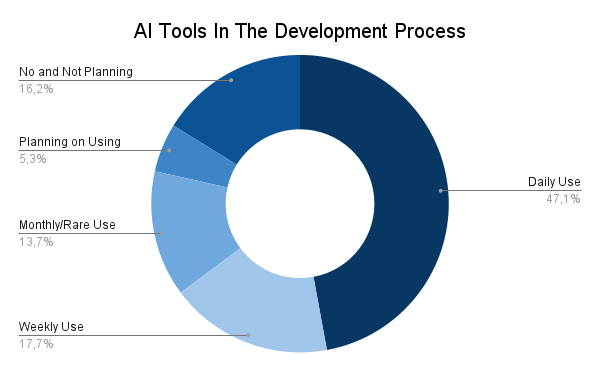
\includegraphics[width=0.88\linewidth]{images/AI Tools In The Development Process.png}
    \caption{Percentage of Users Using AI (Source: Stack Overflow Developer Survey 2025 \cite{stackoverflow2025}).}
    \label{fig:PeopleAI_Graph}
\end{figure}

As we can see in Figure \ref{fig:PeopleAI_Graph} more than 45\% of people that took part in this survey use AI on a daily basis. 
Let's also notice that \textit{more} than 80\% of developers have already integrated or are planning on integrating AI in their programming life.
\end{multicols}



\section*{Survey's Goals}
\addcontentsline{toc}{section}{Survey's Goals}

The goal of this survey to analyze the role that AI tools have in supporting software quality during the process of development. Specifically, it focuses on AI-based systems used for code generation, analysis, and for test automation, without considering chatbots such as ChatGPT or Deepseek.

The objective is to give an overview of these tools, discuss solutions, and to analyze the impact they have on software quality characteristics like maintainability, correctness, and security. As well as, to highlight both the benefits and the limitations of AI-assisted development tools.

\section*{Structure}
\addcontentsline{toc}{section}{Structure}

The survey from this point forward is structured like so. Chapter 1 introduces the background and fundamental concepts related to AI and software quality. Chapter 2 provides a short classification of AI tools used in programming. Chapters 3 through 5 go through code generating AIs, code analysis AI, and test automation AIs respectively. Finally chapter 6 discusses the future directions and open challenges that enabling AI in software quality holds.

\chapter{Background and Fundamental Concepts}


\section{Software Quality Models (ISO/IEC 25010)}

What is ISO/IEC 25010? According to Helpware.tech, ISO/IEC 25010 is a quality model that determines which characteristics to consider when evaluating the quality of a piece of software, whether its still in it's development phase, or even after it has already been released. 

This model consists of 8 different categories defining the quality of a software, from usability and reliability, to security and maintainability among others. These are the main categories this survey is going analyze and take into consideration when overviewing the AI tools.\cite{Quality}

\section{Technical Debt}

The term \textit{technical debt}, in software engineering, describes the cost that comes over periods of time from a suboptimal design or bad implementations that were made during the development phase. Such decision are usually for faster delivery of the product or for a less intense development effort, but usually results in a higher need of maintenance over time.

This phenomenon can happen for various reasons, such as missing documentation and comments, lacking testing, or a poorly structured code. Even though its not necessarily bad, an out of hand technical debt can affect the reliability and maintainability of a piece of software.

In our topic, AI-assisted development, technical debt becomes even more important. Due to automatically generated code, which prioritizes short-term functionality over long-term, if no proper human review is conducted the technical debt can accumulate, and so making future debugging more complex.

Because of this, technical debt is a concept that should be taken in consideration when long-term of AI in software engineering is analyzed.

\section{AI in Software Engineering: Definitions}

In software engineering, the term \textit{artificial intelligence} refers to computing systems designed to support tasks that are typically needed by humans. Some examples include patter recognition, decision-making and problem-solving. Unlike rule-based approaches, AI-based systems rely on data-based methods to adapt to multiple contexts.

Modern AI tools in software development are, more often than not, based on \textit{machine learning} techniques. Machine learning (or ML for short) models are trained on large datasets, often containing source code and the related documentation, in order to learn syntactic and semantic patterns. These models allow for tasks such as code completion, analysis, and automated recommendations.

In this survey the expression \textit{AI-based development tools} is used to describe tools that use AI techniques to help programmers during the development cycle. These tools are not made to operate autonomously, but to support programmers by giving suggestions, analyses, or automated actions.

This leads to AI being adopted in software engineering within a \textit{human-in-the-loop} paradigm, in which developers maintain control over the final decisions. This means that the effectiveness of these tools depends, not only on the quality of the models itself, but also on how the feedback they give back is interpreted and applied in practice.

\section{Ethical \& Legal Aspects in AI-Generated Code}

The use of AI in software engineering introduces ethical and legal challenges that is important they are considered along with the benefits. Particularly, the use of AI code generators may raise concerns regarding code ownership, responsibility as well as data privacy.

The most important legal issue has to do with copyright and intellectual property. Most AI models are trained on publicly available source code, often under different types of licenses. As a result, people wonder about the ownership and the legality of AI produced code.

Accountability is another important aspect to consider. When an AI tool applies directly changes to the source code, it's unclear who's responsible for bugs, vulnerabilities, or failures. Despite that, the final responsibility usually remains with the human developer, who's job is also to review and validate what an AI tool might've suggested.

Because of this, ethical and legal considerations play an important role in introducing AI tools. Reviewing these tools requires more than just a technical analysis, awareness of the risks they bring and their implications in professional development environments is also necessary.



\chapter{AI Tools Classifications}

The AI tools used in software development can be categorized in different groups based on what development aspects they aim to support. This classification exists to clarify the role of every tool, as well as, give a more structured analysis on the impact they have on software quality.

In this survey, the AI tools have been classified in three main categories: Code generating AIs , code analysis AIs, and test automation AIs. Each one of these dresses different challenges related to software quality, from to productivity and correctness all the way to maintainability and reliability.

The next sections introduce these categories and mention their main characteristics, laying the groundwork for the detailed analysis that follows in the next chapters.

\newpage

\section{Code Generating AIs}

Code generating AIs are one of the most broadly known category of AIs when talking about software development. Such tools help developers by producing code suggestions based on contextual information provided by the programmer and the surrounding code, and their main objective is to reduce the probability of human errors in a program. 

While these tools can help improve productivity, the impact they have on software quality is not always straightforward. Generated code usually contains logical errors, security issues or a reduced readability if it's not reviewed properly. Because of this, these tools are most effective when in use within a human-in-the-loop workflow, rather than in a fully isolated environment.

\section{Code Analysis AIs}

Code Analysis AIs expand on the previously mentioned reduction of human error in a program, their objective is to inspect the written code, whether that being AI or human generated, for any problems, violation of coding standards, as well as to detect and fix any bugs that might be present in the structure of the software, usually relying on a combination of static analysis techniques and ML models.

By examining large codebases, code analysis AIs aim to improve the maintainability throughout the development cycle. However, their effectiveness relies on how accurate the analysis is and how well the developers interpret the reported issues.

\section{Test Automation AIs}

Test automation AIs main goal is to help the software testing process by generating, executing, and prioritizing test cases. These tools aim to increase test coverage and to discover the execution paths that may be overlooked during human testing.

While these AI tools can help enhance reliability, the quality of the tests they generate depends on the models they use and datasets available. This means that, human supervision is more often than not required for the validation of the tests and also, to ensure that critical scenarios are also covered.

\chapter{Code Generating AIs}

Code generating AI tools are probably the most prominent application of machine learning in today's software development. They are a category of AI-based development tools which aim at assist developers by automatically producing code-based on the contextual information. Their constant raise in working environments has raised concerns about their potential impact on the software's productivity and quality.

Even though, these tools can help accelerating development and reduce mundane tasks, they also bring forward challenges regarding  maintainability and security. AI generated code could contain small logical error or even vulnerabilities difficult to recognize without human verification. This is why knowing what they can and can't do is essential when introducing them in software development.

This chapter's purpose is to provide an overview of code generating AIs, such as GitHub Copilot, Claude and Cursor. We'll analyze how these tools operate, how they are used in practice ,and the impact they have on software quality and reliability.

\newpage

\begin{table}[h]
\small
\centering
\caption{Feature-based comparison of selected Code Generating AIs}
\resizebox{1\textwidth}{41pt}{
\begin{tabular}{|c|c|c|c|}
\hline
\textbf{Feature} & \textbf{GitHub Copilot} & \textbf{Cursor} & \textbf{Claude}\\
\hline
\textbf{Primary purpose} & Inline code completion \& suggestions & Project-wide code editing \& generation & Large-scale code generation \\
\hline
\textbf{Context awareness} & Limited to opened files & Full project via workspace indexing & Large context window (project-level) \\
\hline
\textbf{IDE integration} & VS Code, JetBrain IDEs, Neovim & Standalone IDE (Based on VS Code) & Web interface / IDE plugins \\
\hline
\textbf{Test generation} & Limited & Prompt-based & Prompt-based \\
\hline
\textbf{User interaction} & Continuous inline suggestions & Command-based & Prompt-based \\
\hline
\textbf{Target audience} & Individual developers & Individual developers \& small teams & Individual developers \\
\hline
\end{tabular}
}
\label{table_3.1}
\end{table}

Table \ref{table_3.1} provides an overview of the main characteristics of the code generating AIs that are considered in this survey, as well as they are used and integrated in the development cycle.

\section{GitHub Copilot}

GitHub Copilot is an AI for code \textit{completion}, released in October 2021, developed by GitHub with the assistance of OpenAI, and it is integrated in various IDEs such as Visual Studio Code, NeoVim, and even JetBrains to mention a few\cite{Copilot}. 

In the beginning Copilot just used OpenAI's GPT\cite{CopilotAPI} but, ever since 2024, it has expanded to include Anthropic's Claude, and even Google's Gemini. According to GitHub, Copilot's main purpose is to help developers get accustomed to new coding frameworks by reducing the time spent reading documentation.

The way that Copilot works is by collecting pre-existing code, written and uploaded onto public GitHub repositories by programmers, and then starts suggesting code snippets which auto-completes our coding when writing it. It can even convert code comments to runnable code and autocomplete repetitive sections, as well as methods and functions.

It is to be noted that even GitHub mentions how Copilot managed to autocomplete correctly roughly half of the times; When given a Python header code it was correct 43\% of the times on it's first attempt and raising to 57\% of the times after ten attempts\cite{CopilotFAQ}.

From a software quality point of view, Copilot could improve the development speed, but it may also introduce hidden errors or reduce the clarity of the code if it is not properly reviewed. As a result, its effectiveness depends on the developer's experience and critical evaluation.

\section{Claude and Claude Code}

Claude is a Large Language Model developed by Anthropic with it's first release being on March of 2023 with Claude 1 and the latest, Claude Opus 4.5, in November of 2025. 

\begin{figure}[H]
    \centering
    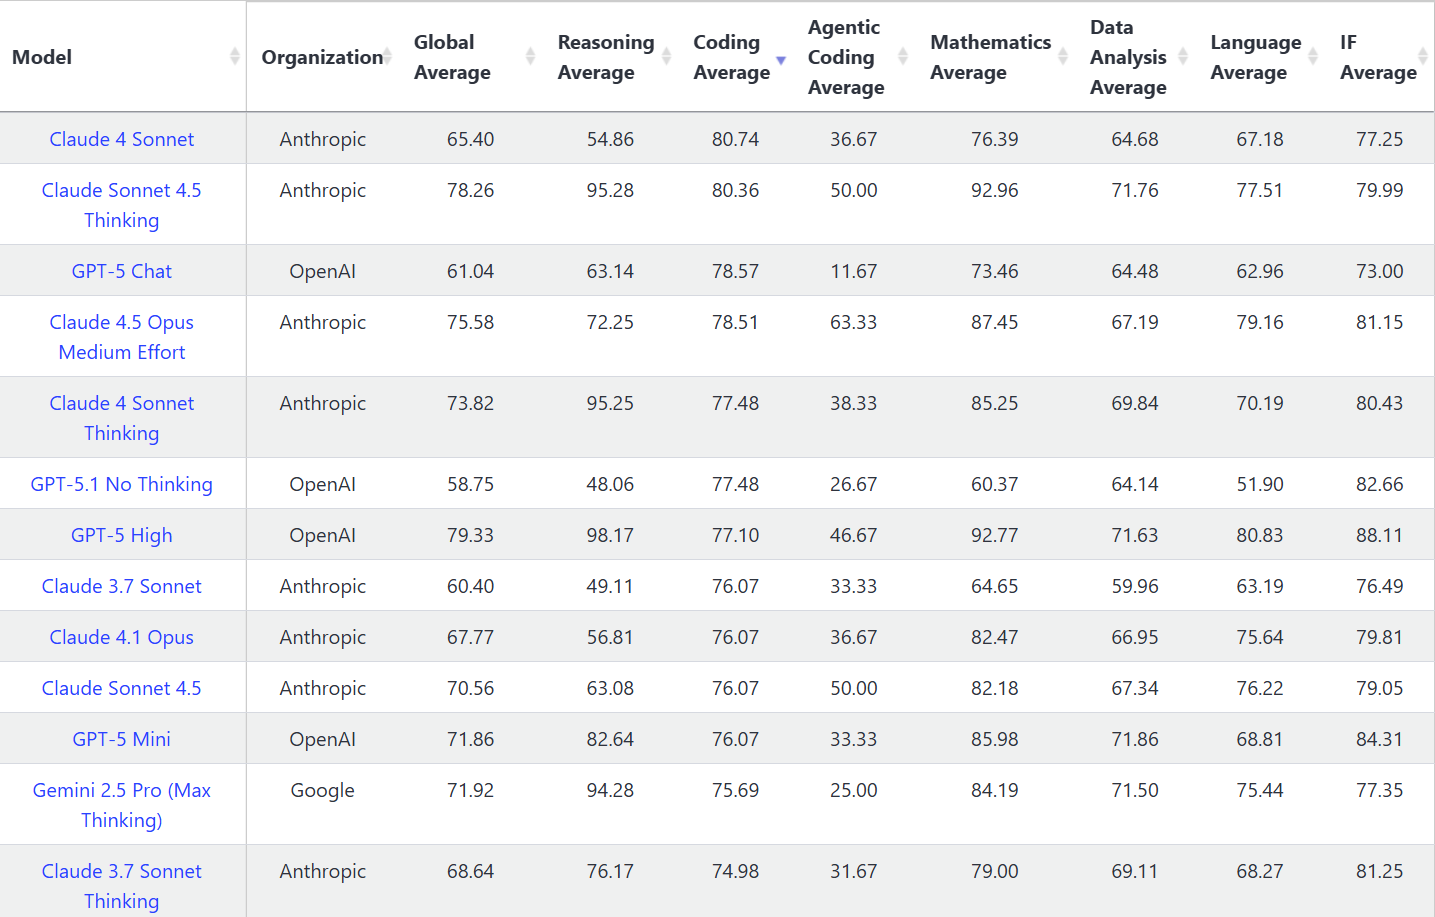
\includegraphics[width=0.95\linewidth]{images/Screenshot 2025-12-23 214938.png}
    \caption{LLMs Benchmark - Coding Average \cite{livebench}}
    \label{fig:AI_Benchmark}
\end{figure}

When Claude first came out coding wasn't one of it's most proficient skills. But now, unlike it's other counterparts, coding has become it's strongest suit, as we can see from this benchmark made for LLMs (filtered by "Coding Average") in which Claude models manage to get the top spots on the leaderboard followed \textit{only} from OpenAI's newest model.

Unlike tools like Cursor and GitHub Copilot, Claude is more often than not accessed through a conventional prompt-based interface, with the possibility to add it to your IDE through plug-ins, which changes the way the tool is used in software engineering. Programmers usually prefer a more traditional interaction, instead of receiving inline suggestions during coding. This type of interaction encourages a deeper reasoning.

Quality wise, Claude has the possibility to help improve code readability by explaining to the programmer what the logic behind given code snippets is. It's important to know that the quality of the output depends almost entirely on the prompt the developer gives, which shows how important human reviewing is when such tools are introduced in software development.

\section{Cursor IDE}

Cursor is an Integrated Development Environment with an LLM embedded in it. It was released in 2023, a little over two years ago, and it just recently had it's first stable release, Cursor 2.0, which came out on October 29th 2025.\cite{CursorRelease}. 

\begin{figure}[H]
    \centering
    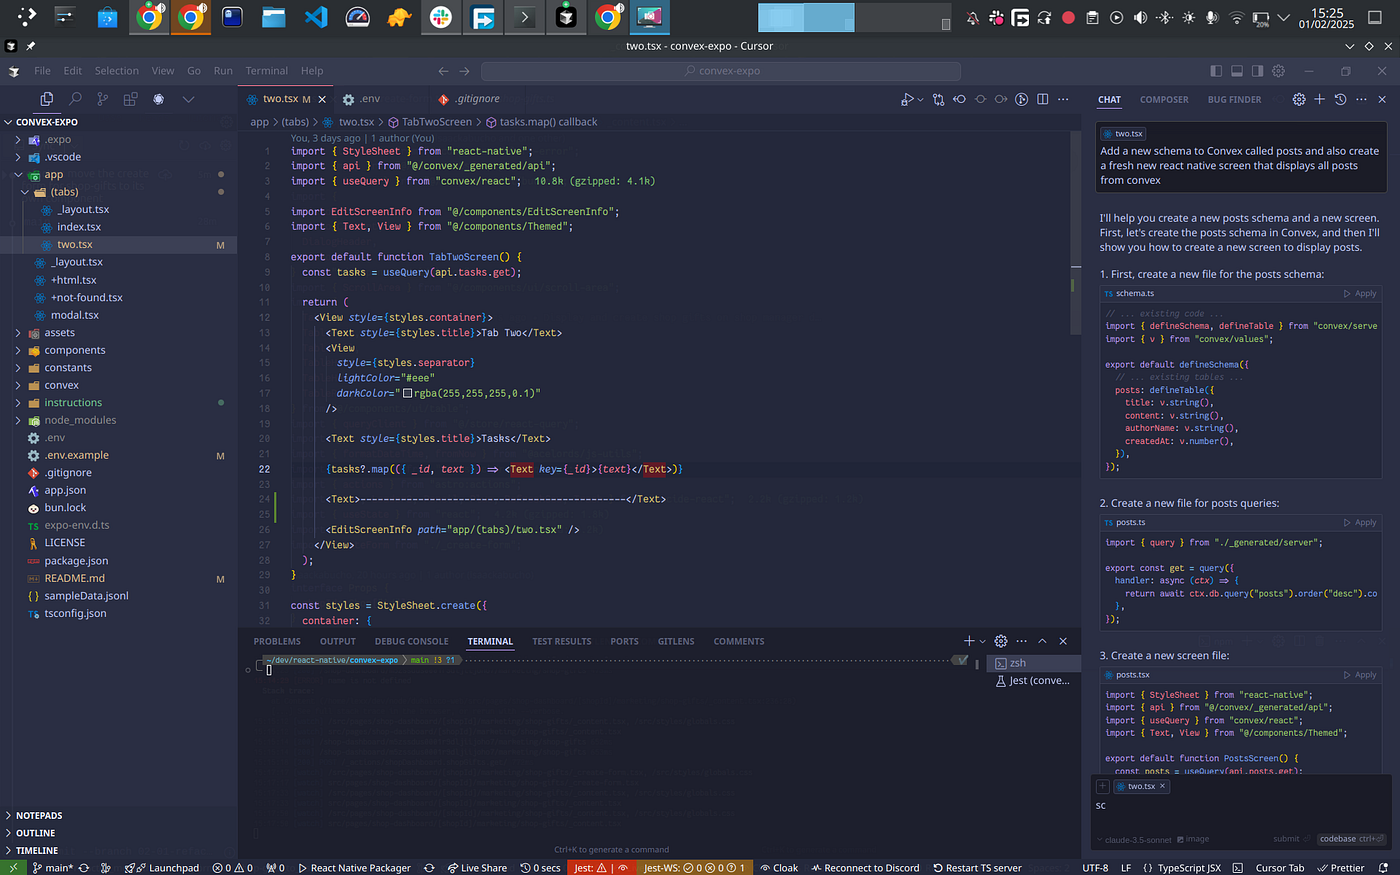
\includegraphics[width=0.95\linewidth]{images/1_P0MD8MiEGvIEdNFZpfkm5Q.png}
    \caption{Cursor IDE GUI \cite{CursorGUI}}
    \label{fig:Cursor_IDE}
\end{figure}

It was made as a fork of the Visual Studio Code IDEs\cite{VSCodeIDE}, and as such the transition from one IDE to the other is smooth and easy, which has made many developers start to switch from VSCode, but also from other unrelated IDEs, to Cursor due to its AI integration and quality of life features such as error detection and automated fixing that the environment offers, as well as the automatic code generation from a user generated prompt.

Of course, such a tool comes with its flaws. As mentioned by Yulia Kumar and her colleagues\cite{kumar2025evaluating}, Cursor can be a double-edged sword: it helps you find the problem and fix it, but it will not explain \textit{why} it does what it does. This means that as programmers we went from not understanding how the code works to not understanding how an error got fixed. They also mentioned that people with no prior coding experience were able to learn the IDE in just four days, code a functioning app in just three weeks, but needed an additional six weeks just to understand what the LLM had written. 

\chapter{Code Analysis AIs}

Code Analysis AI tools are Ai-based development tools designed to aid developers in evaluating their code in order to detect potential problems and suggest corrections. Unlike Code Generating AIs, these tools focus on analyzing and reviewing code that's already been written instead of generating their own. Their goal is to support software quality with bug-detection, enforcing coding standards, and bringing up areas that could affect maintainability or security.

The use of these tools has been increasing in recent years, this is due to software systems becoming more complex and harder for humans \textit{alone} to maintain. These AIs reduce human efforts by automating some of the review and analysis process while still providing feedback. Even so, their effectiveness depends on the accuracy of the analysis they provide and on how programmers interpret it and apply the corrections.

This chapter gives an overview of code analysis AI tools and discusses some selected systems such as Qodo, CodeRabbit, and CodeAnt AI. The analysis focuses on their main functionalities, modes of integration, and their impact on software quality.

\newpage

\begin{table}[h]
\small
\centering
\caption{Feature-based comparison of selected Code Analysis AIs}
\resizebox{1\textwidth}{41pt}{
\begin{tabular}{|c|c|c|c|}
\hline
\textbf{Feature} & \textbf{Qodo} & \textbf{CodeRabbit} & \textbf{CodeAnt AI}\\
\hline
\textbf{Primary purpose} & Automated code review & Code quality assessment & AI-driven code analysis \\
\hline
\textbf{Type of analysis} & Static code analysis & Static with quality metrics & Static with machine learning techniques \\
\hline
\textbf{Bug detection} & Detection of common bugs & Detection of bugs \& code patterns & Detection of bugs \& anomalous code patterns \\
\hline
\textbf{Integration environment} & IDEs \& pull requests & IDEs \& repository platform & IDE focused \\
\hline
\textbf{Feedback timing} & Post-analysis review & Post-analysis review & Real-time feedback \\
\hline
\textbf{Security-related analysis} & Limited focus & Not primary focus & Detection of security issues \\
\hline
\textbf{Refactoring support} & Limited \& descriptive & Explicit suggestions & Automated \& context-aware suggestions \\
\hline
\textbf{Use of Machine Learning} & Rule based \& ML-assisted analysis & ML assisted analysis & ML assisted analysis \\
\hline
\end{tabular}
}
\label{table_4.1}
\end{table}

Table \ref{table_4.1} shows how AI code analysis tools are differentiated, not just by their functional scope but also by the level of automation and by the role that machine learning plays in the review process. 

\section{Qodo}

Founded in 2022 with the name \textbf{Codium}, Qodo's main focus is to make sure the code quality in multi-repo environments is enforced, so that bigger teams manage to ship software faster and more reliably\cite{qodo}. It's mainly designed for organizations in which multiple programmers work on complex databases.

Qodo works by using AI to provide deep and thorough code analysis during the whole development of a piece of software by being innately integrated in the programmer's IDE and pull requests. It can learn company standards and align its recommendations with the company conventions once it has received enough information on what its expected or needed.

Software quality wise, Qodo helps improve the maintainability and reliability of the source code. It helps reducing technical debt and promotes uniform coding practices by analyzing how the code is modified and by constantly enforcing standards, so that issues can be addressed before deployment and end up with a more stable end-result.

On the other hand, programmers need to keep validating the recommendations that Qodo gives for them to be effective, this reinforces the importance of humans reviewing code analysis AIs.

\newpage

\section{CodeRabbit}

Founded in early 2023, CodeRabbit's purpose is to aid developers to find mistakes in their programs, it achieves this by scanning the source code, find bugs, suggest solutions, and elaborate on possible consequences if something is not fixed. Once it's in a programmer's cycle it can access and review pull requests, help a team review code and ship pieces of software faster, with fewer bugs making it in the final product\cite{CodeRabbit}. 

\begin{figure}[H]
    \centering
    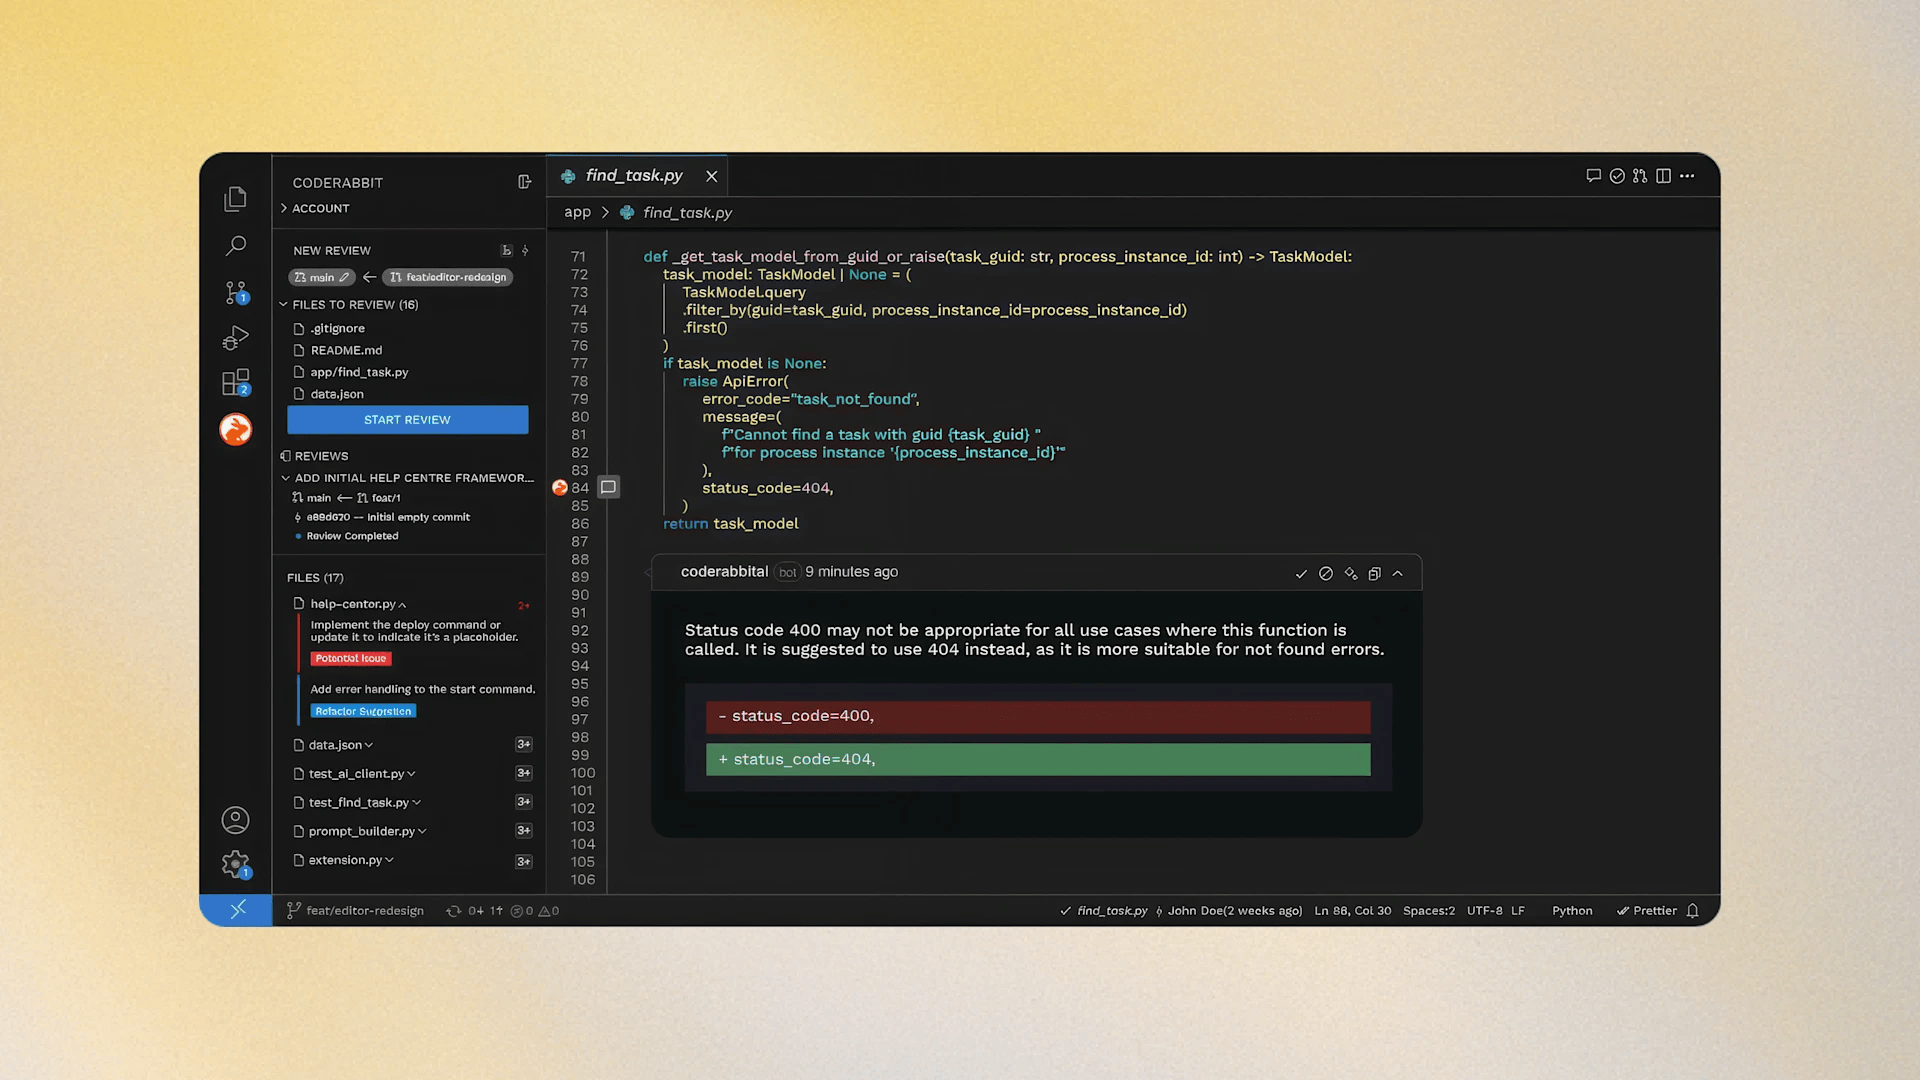
\includegraphics[width=1.081\linewidth]{images/oai_Coderabbit_UI_asset_16x9.png}
    \caption{CodeRabbit suggestion in IDE\cite{coderabbit_ui}}
    \label{fig:coderabbit_1}
\end{figure}

CodeRabbit uses AI to analyze ho source code changes in various pull requests, allowing for feedback to be provided beyond simple syntax. The suggestions it offers are accompanied by explanations, helping developers get a better understanding behind both the issues and the solutions.

In software quality terms, it helps identifying bugs early in the programming cycle, this tool reduces the chances of having faulty code being merged in the main branches of a program. In addition to that, the emphasis on contextual feedback can help development teams share knowledge, leading to better programming practices over time.

Nevertheless, just like with various code analysis AIs, the responsibility of accepting or not the various suggestions \textit{always} remains with the humans overlooking the tool.

\section{CodeAnt AI}

CodeAnt was founded as software startup in 2023 San Francisco, California\cite{CodeAnt}. It's designed to help developers identify the quality and safety issues inside the code. It's purpose is to analyze codebases and to find vulnerabilities, bugs, and structural problems that may affect maintainability. Unlike code generating tools, CodeAnt AI focuses on improving the quality of a piece of software by evaluating and refining already written code.

\begin{figure}[H]
    \centering
    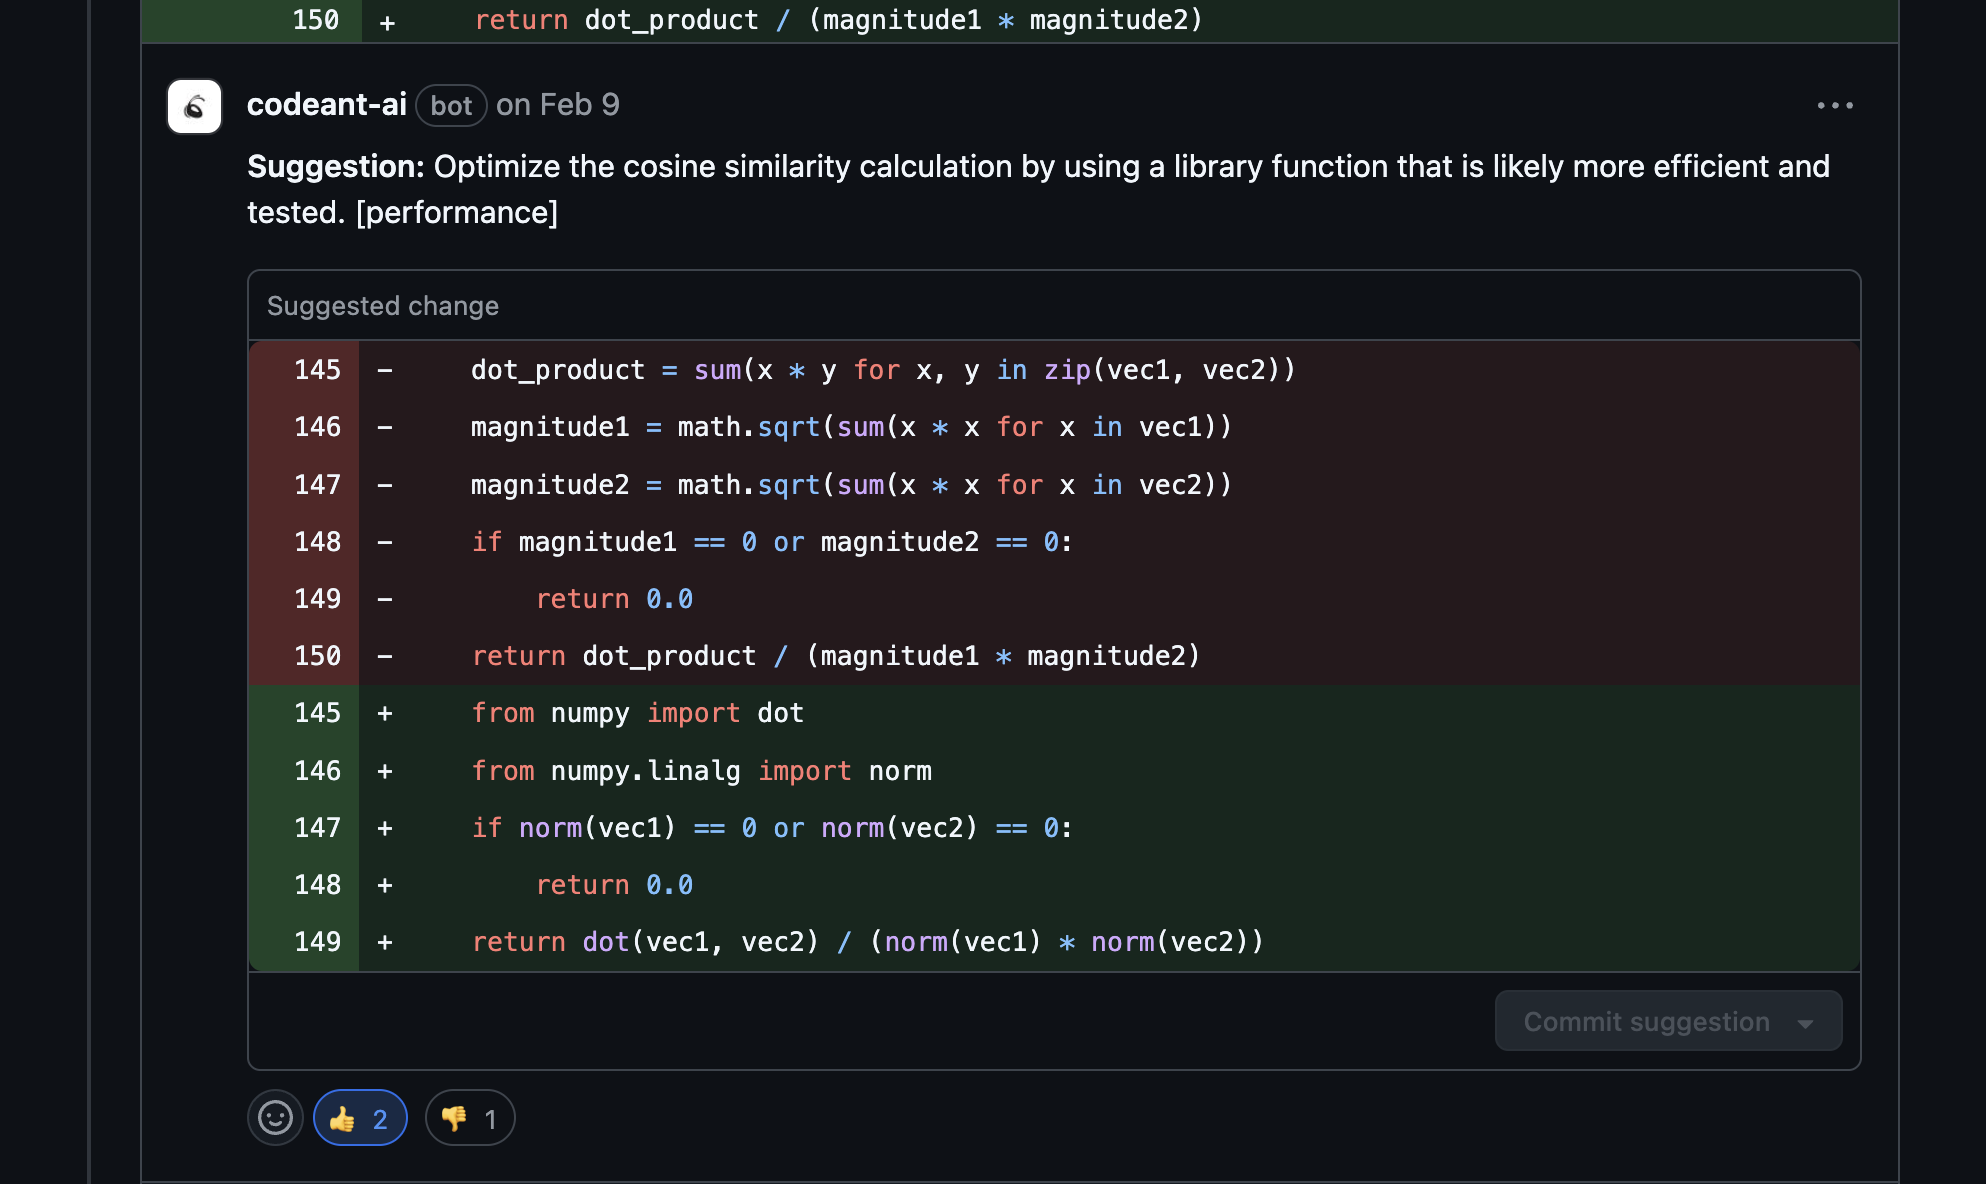
\includegraphics[width=0.9\linewidth]{images/ai-code-review-in-action.png}
    \caption{CodeAnt suggestion in IDE\cite{codeant_ui}}
    \label{fig:codeant_1}
\end{figure}

CodeAnt main concerns are software security and maintainability. Through an automated analysis, it shows weaknesses that be the reasons behind security problems or technical debt if left unattended. Because of this, especially when its done in the early stages of programming, the tool becomes important when reliability and compliance are a major goal and it also help developers maintain a cleaner and sustainable code structure in the long run.

When analyzed from a software quality point of view, CodeAnt's objective is to improve the maintainability and structure of a program, the detection of problems in the early stages lets teams fix them before they propagate throughout the system.

However, even in this case human intervention is still required when interpreting and validating CodeAnt's suggestions, reinforcing the programmers' role in quality decisions and making the final design.

\chapter{Test Automation AIs}

Testing software is an incredibly important factor when talking about software quality, it's objective is to verify that the code structure works as intended while also detecting problems before deployment. However, traditional testing procedures are usually time-consuming, require a lot of work, and are difficult to maintain especially in today's age where software systems keep rapidly evolving. Because of this, test automation has become a necessary component in modern programming.

Recently, AI has been introduced to test automation with the main objective of improving the effectiveness of such tests, while also reducing the effort required. AI test automation tool use various techniques, such as machine learning and pattern recognition to create, execute, and maintain test cases.

Software quality wise, test automation AIs have the possibility of increasing test coverage and enhancing the detection of problems. On the other hand, the use of these tools brings forward new hardships, such as an appropriate and in-depth validation of the test results by a human and the risk of relying on the tools too much. Knowing both the pros and cons of test automation AIs is necessary when we look at the impact it'll have on software quality.

\begin{table}[h]
\small
\centering
\caption{Feature-based comparison of selected Test Automation AIs}
\resizebox{1\textwidth}{41pt}{
\begin{tabular}{|c|c|c|c|}
\hline
\textbf{Feature} & \textbf{mabl} & \textbf{Testim} & \textbf{Testsigma}\\
\hline
\textbf{Primary purpose} & End-to-end web testing & End-to-end web \& mobile testing & End-to-end web \& mobile testing \\
\hline
\textbf{AI Usage} & Test generation & Smart locators & NLP-based test execution \\
\hline
\textbf{Test types supported} & Functional, regression & Functional, regression & Functional, regression \\
\hline
\textbf{Developer control} & Medium & High & Medium \\
\hline
\textbf{Accessibility} & Medium & Medium-high & High \\
\hline
\textbf{Suited for} & Automated regression pipelines & Controlled AI testing & Accessible test automation \\
\hline
\end{tabular}
}
\label{table_5.1}
\end{table}

\newpage

\section{Mabl}

Mabl is an AI-native test automation platform founded in 2016, with the objective of empowering software teams to deliver high quality software. \cite{mabl} Using its CLI developers can execute tests locally, this lets them get sooner during programming a feedback before their work is merged on the main branch of a project.


\begin{figure}[H]
    \centering
    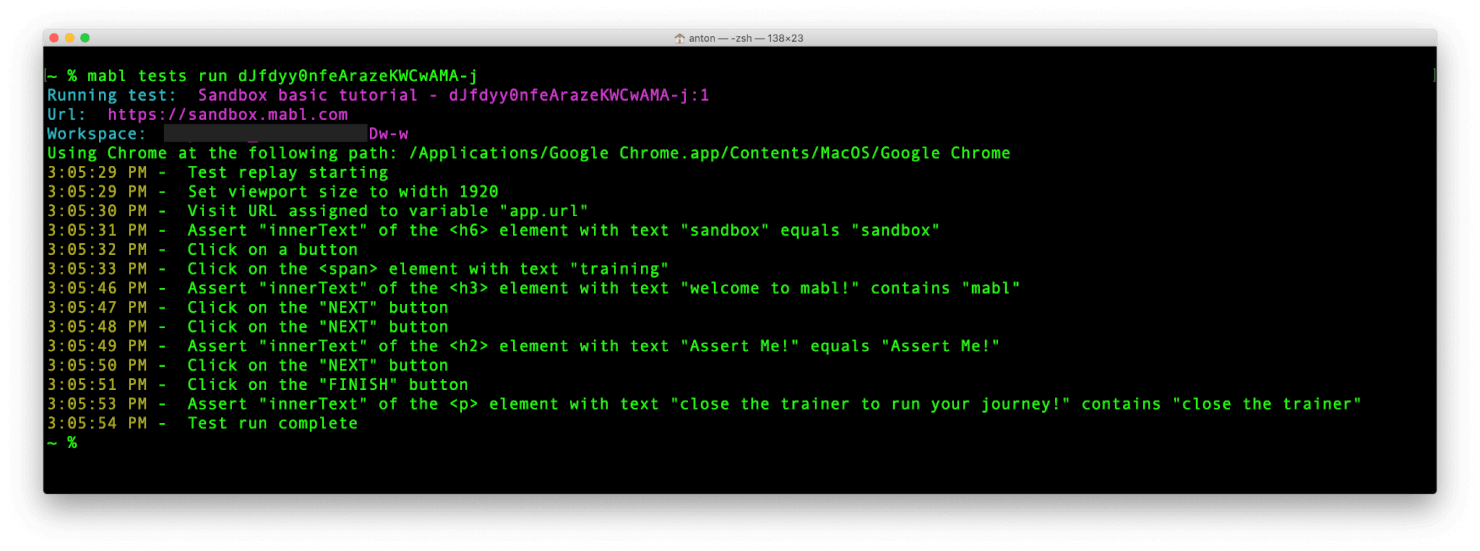
\includegraphics[width=0.95\linewidth]{images/mabl1.png}
    \caption{Executing and monitoring tests from terminal with mabl CLI \cite{what_is_mabl}}
    \label{fig:mabl_1}
\end{figure}

One of the main features of mabl is how it uses AI techniques to adapt test cases to changes in the program while testing. Through various mechanisms, mabl has the ability to modify codes in which UI elements might be changing reducing how fragile a test might be. In addition to that, mabl can create a customized test automatically based on the user's interactions or necessities.

When viewed under how it impacts on software quality, mail's main objective is to make sure that the reliability and regression testing effectiveness is improved. Since it maintains the test validity long-term it makes sure that if there is a change in the source code it wont lead to unwanted side effects. However, programmers could understand the test logic less because of the \textit{abstraction} that mabl offer, which means that a careful validation of the results is mandatory.

In the end, even though mabl offers some great advantages we should also look at the limitations it comes with. Relying too much on an automated test generator could make it so that programmers aren't in control of ho the tests behave, especially in more complex scenarios. In addition to that, an oversight of quality of the data used to train the AI is necessary to increase its effectiveness.

\section{Testim}

Testim is a full-featured test automation platform, launched in the late 2014 and with the objective of turning the mundane procedure of hand writing end-to-end tests into an AI-based functional test automation solution\cite{what_is_testim}. It's designed to be integrated in today's development cycles, supporting constant testing.

\begin{figure}[H]
    \centering
    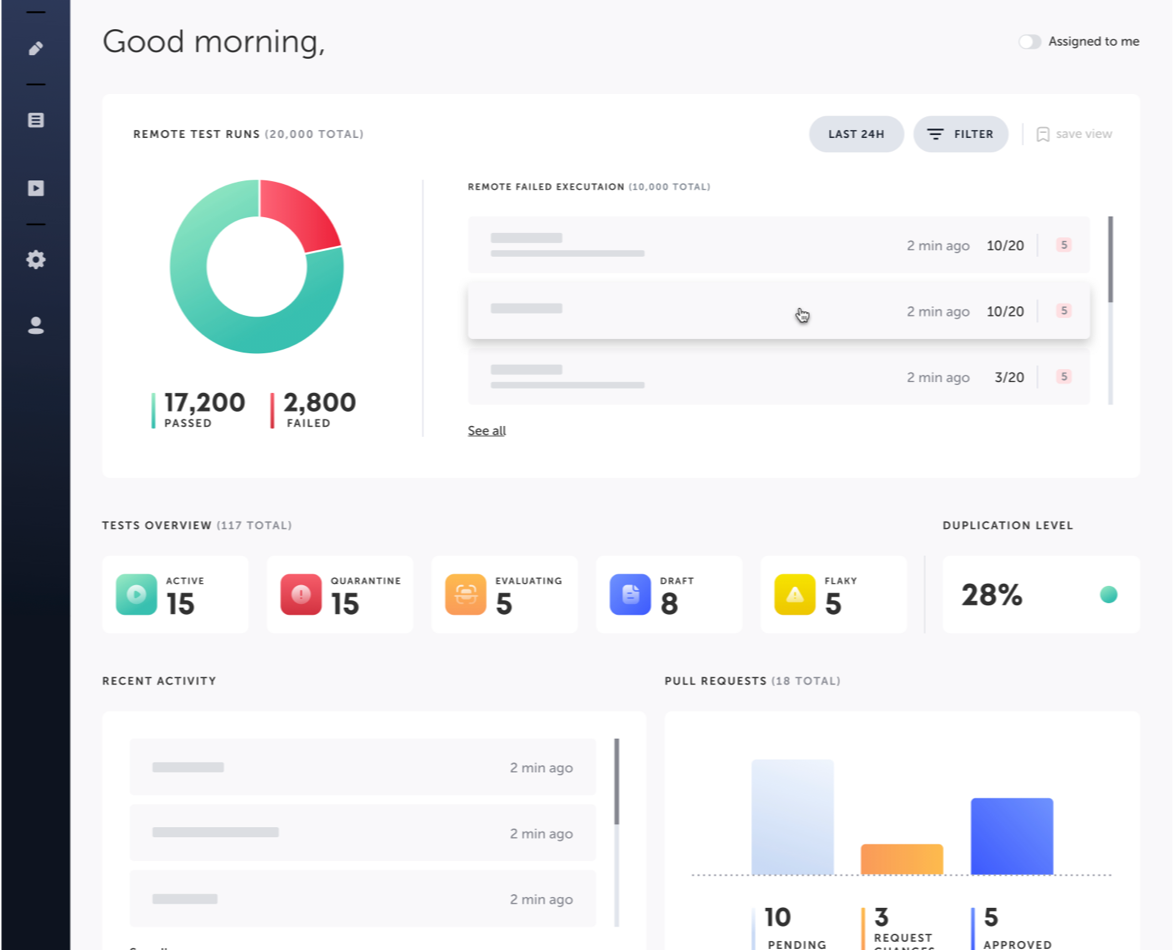
\includegraphics[width=0.55\linewidth]{images/dashboard_carousel@2x-1174x950.png}
    \caption{Testim UI \cite{testim_ui}}
    \label{fig:testim_1}
\end{figure}

It uses AI locators which make the creation of tests an easier task while also keeping them working when the source code gets modified. In addition to that, customized locators, that are made specifically for your application, are also one of the main methods used by Testim. It can also group automatically for reusable modules, for example it can save time with the creation and maintaining of duplicate tests and also identify steps that are repeated and can then be reused. \cite{what_testim_does}

Software quality wise, Testim contributes on making automated tests while making sure their reliability and maintainability is improved. It can reduce the amount of false-alarms when an interface change is done since it supports a stable regression testing process. Another positive is that Testim lets you customize the logic behind a test which lets programmers remain in control, unlike other test automation AIs.

Even though Testim has many advantages, there also are some important limitations to be taken in consideration. While the previously mentioned locators can improve complex scenarios it still \textit{needs} manual scripting and some tuning by a human. Additionally the effectiveness is strictly dependent on the quality of the recorded test, highlighting how important the test design and validation is.

\section{Testsigma}

Testsigma is a test automation platform, launched in 2019, with the purpose of making automated testing for mobile apps, web testing, and APIs an easier task. It's main user base is composed of startups and product teams, making sure they're able to make and manage tests in plain English \cite{testsigma}.

\begin{figure}[H]
    \centering
    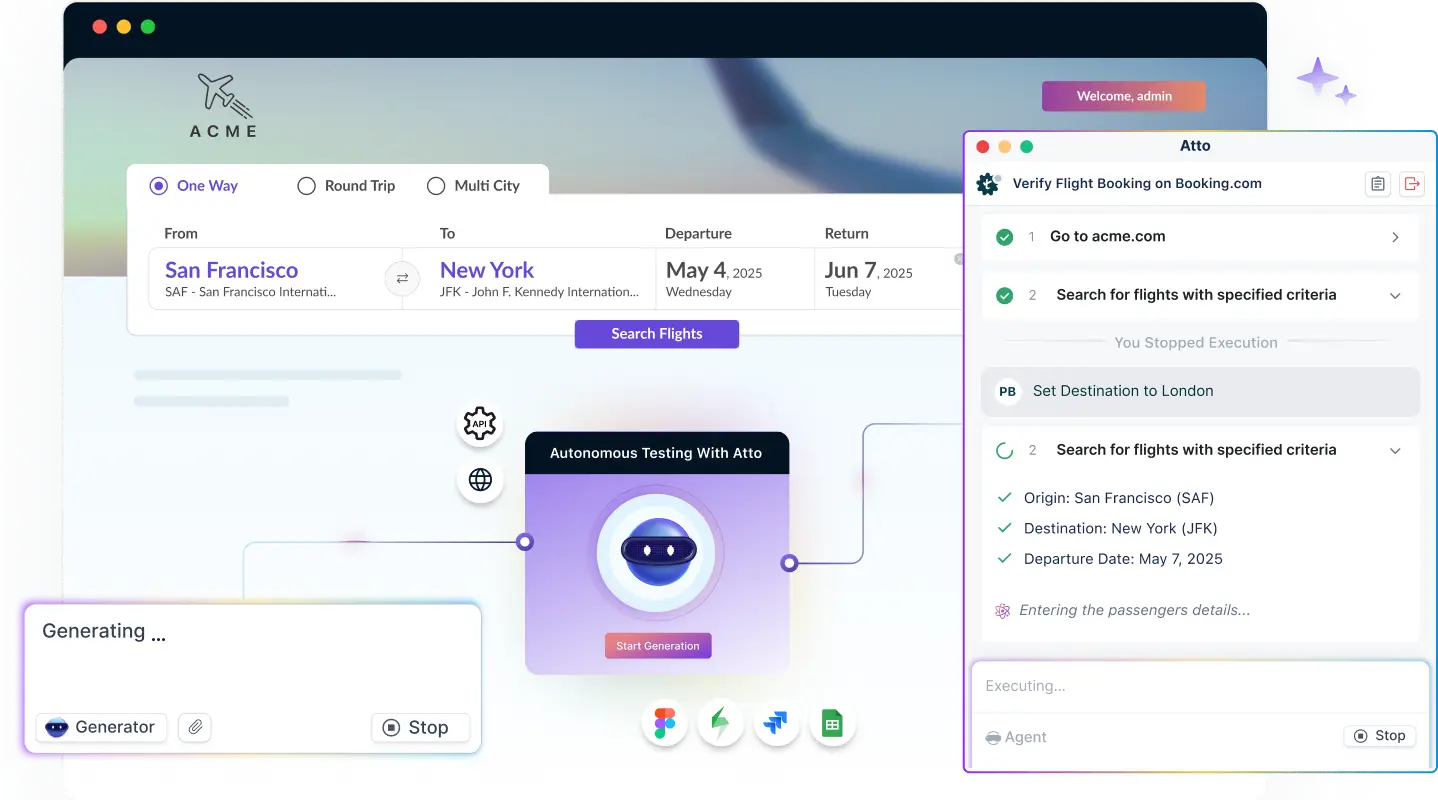
\includegraphics[width=0.77\linewidth]{images/ai-web-testing.png}
    \caption{Testsigma UI with an example of English written test \cite{testsigma_ui}}
    \label{fig:testsigma_1}
\end{figure}

It applies AI to make test creation, execution, and maintenance an automatic procedure. Like we saw in the Figure \ref{fig:testsigma_1} the steps are written in a classic language (such as English), which means that the use of traditional scripting languages is reduced. Like Testim, it uses AI-based mechanisms to adapt the tests when the applications are modified, and it also supports cross-browser and platform testing with little to none intervention. \cite{testsigma}

When we talk about software quality, Testsigma supports an improved test coverage and consistency. Since it makes the test creation a less complex task, it enables a broader participation during the testing phase, which may lead to a higher number of validated scenarios. This helps detect bugs early on and also have more reliable regression testing.

On the other hand, using Testsigma comes with some limitations. Due to the natural languages prompts the control over the behavior of the test is reduced, making it not ideal for more complex scenarios. In addition to that, the excessive use of natural languages can limit the flexibility when compared to a script-based testing approach.

\chapter{Future Directions}

\section{Measuring the Impact of AI on Software Quality}

Measuring the impact of AI based tools on software quality remains an open challenge. Software quality is a complex concept that includes factors like maintainability, reliability, and security, which are often difficult to evaluate by themselves. Despite the existence of quality models, like ISO/IEC 25010, which provide a useful framework. Applying them consistently to AI assisted development workflows remains an ongoing research.

The evaluations of AI tools done now usually rely on productivity metrics or short-term studies. Even though these approaches can give an insight in specific capabilities, the could not be able to capture the long-term effects that AI assistance has on software quality. A great example we know is that, a greater development speed does not mean that the final product will be of higher quality, or even easier to maintain.

One more limitation is found in the lack of standardized evaluation methodologies. Different studies would focus on \textit{singular} aspects of quality, like code correctness or even bug detection. This makes comparing multiple tools' results a complicated task.

Future studies should include the development of more comprehensive evaluation frameworks. Researches involving development teams could provide insight on the influence AI-based tools have on software quality. These actions may help close the gap between controlled experiments and practical programming outcomes.

\section{Long-Term Maintainability and Technical Debt}

The effects that AI-tools have on software quality, long term, remain an open discussion. Even though these tools can improve a code structure, as well as the productivity of it, on a short-term basis, on a long-term on the influence they have over the structure and the constant evolution of programming is less understood. Maintainability, but also code readability, ease of modification and safety, could get affected by the assistance of AI.

A big concern is the accumulation of \textit{technical debt}. Generated code could prioritize functional over logical correctness, we can see this happen when developers rely on AI and adopt the suggestions given without properly understanding their significance. This will inevitably lead to codebases that are harder to debug, modernize, or refactor, increasing the need for maintenance over time.

On the other hand, these tools can also positively enhance the quality over long periods of time by encouraging standardized coding practices and by identifying quality-related issues early during the development phase. For example, automated detection of bugs or complex structures can help reducing the growth of technical debt.

Future studies should aim at figuring out the impact that AI-assisted programming has on extended period of time. Analyzing code evolution, cost of maintenance, and the developer comprehensions are all studies that could give insights on if AI-tools can mitigate the technical debt in real-word coding projects.

\section{Human Oversight and Trust in AI Tools}

With the increase of AI-based tools in development we see how important the concepts of human oversight and trust are. While AIs are able to provide assistance in tasks like code generation, analysis and testing, there is always a risk that their outputs are incorrect or even just suboptimal. As a result, relying on AI without evaluating the result given can lead to risking the software quality.

Trust in AI tools plays a significant role in the programming cycle. Excessively trusting such tools can often lead to the programming relying on them too much, often accepting generated suggestions without a proper check. On the other hand a lack of trust can reduce the benefits of having AI \textit{assist} the programming experience, limiting its effectiveness. A balance between trust and skepticism is incredibly important to achieve.

Human-in-the-loop methods are a promising directions that should be maintained. By having developers still actively involved in decision-making, it ensures that AI systems work as expected but most importantly as supportive tools rather than a replacement. Some features that AIs offer, and should be taken in consideration, like transparency over the thought process, explained suggestions, and customization levels of assistance may help programmers understand and evaluate better AI-generated recommendations.

Developments in the future should aim on making AI tools that cultivate meaningful human oversight and informed trust. Improving the explainability and providing a clearer feedback may help developers make more responsible decisions while also, enhancing the reliability of AI-assisted software systems.

\section{Ethical AI for Software Engineering}

The rise of AI in software engineering raises ethical questions beyond the technical performance. As these tools influence code generation, analysis, and testing, questions related to responsibility and transparency start to become more relevant. This means that Ethical AI in programming requires a careful consideration of how the tools are designed, deployed, and used practically.

One of the biggest concerns is the \textit{accountability}. When AI systems help software development, it could become unclear as to who's responsible for vulnerabilities, defects, or even unintended behaviors in the code. Despite the use of AI tools, responsibility remains with human developers, as well as with the companies, highlighting the importance for clear instructions and oversights.

Transparency and explainability also play an important role in ethical AI adoption. Programmers \textit{need} to understand, at least to some degree, why the AI tools return certain suggestions. Without a good enough transparency, deciding how reliable an AI-generated output or detecting biases from training data becomes complicated.

In the end, the ethical aspect is closely related to trust and long-term adoption. Tools that don't manage to respect privacy or intellectual property could stop being used, despite advantages that they may have over other tools. In the future, programmers that use AI should make their number one concern the ethical aspect of using such tools.


\chapter*{Conclusion}

As we saw, this survey analyzed the role of various AI tools in supporting software development, mainly focusing on their impact on software quality. By examining various categories, such as code generating, analysis, and test automation, the work aimed to give an overview of how these technologies are being used in today's software engineering practices.

The review highlighted how AI can be a positively used tool in various fields, such as maintainability, reliability, and bug prevention. Code generating tools help the developers' productivity, while code analysis and test automation ones have a more important role in finding bugs, making sure company standards are enforced, and improving the tests effectiveness. It is important to remember, however, that such benefits usually come with multiple trade-offs related to control, transparency, and long-term maintainability.

A theme that could've been found all throughout the survey is how much human oversight is needed. Despite AI tools being able to act autonomously and enhance various steps of the development cycle, their results and recommendations need a careful review by human before being integrated in the main code structure, especially to avoid over-reliance and quality degradation. Because of this, concepts like technical \textit{debt} and \textit{trust} are important  when evaluating the long-term results of using AI in the development cycle

Overall, AI tools should be used in a way that helps programmers and does not replace them. When used properly in workflows and reviewed under the appropriate criteria, they have the potential to make software more reliable and maintainable. A continued research is going to be key for a better understanding on the impact they yield long-term on software quality and development practices.

\bibliographystyle{unsrt}
\bibliography{ref}

\end{document}
